\section{Andamento dei progetti con piu di dieci iterazioni}
\label{sec:results-iteration-trends}
% Evidence: iteration_trends/{iteration_metrics.csv,run_summary.csv,evidence_manifest.json}.
L'analisi seleziona i progetti per cui almeno una configurazione completa
supera dieci iterazioni nel medesimo snapshot dei risultati precedenti.
Sono nove run su sei progetti: sei raggiungono la convergenza e tre
terminano al limite di 25 iterazioni. Per ciascun progetto si riportano
anche le altre configurazioni P0, P1 e P4, comprese quelle piu brevi,
per confrontare le traiettorie dalla stessa gerarchia iniziale.

L'iterazione 0 indica la baseline top-down; ogni valore successivo valuta
lo stato dopo una completa iterazione, incluse rimozioni e riparazioni
effettivamente accettate. Si usa lo stesso scorer BERT, preprocessing e
matching dei risultati finali. Una riparazione rifiutata puo lasciare
invariata la gerarchia e quindi le metriche. Le curve terminano allo stop
effettivo: i trattini nelle tabelle indicano iterazioni non eseguite,
non valori nulli o mancata convergenza.
L'eventuale riconciliazione iniziale dei riferimenti padre--figlio,
registrata dal ciclo, non modifica le descrizioni usate dallo scorer.

Queste traiettorie sono un'analisi descrittiva del processo: non vengono
mediate per ricalcolare le prestazioni finali e non rappresentano repliche
indipendenti. Il sottoinsieme selezionato per durata non descrive da solo
le prestazioni su tutti i dodici dataset. I valori di Precision e Recall,
i conteggi dei goal e delle decisioni per iterazione restano nel CSV
\path{output/evaluation/thesis_completed_v103_20261025/iteration_trends/iteration_metrics.csv}.

\clearpage
\subsection{AUU}
P0: 25 iterazioni, limite raggiunto; P1: 4 iterazioni, convergenza; P4: 18 iterazioni, convergenza.
\begin{figure}[htbp]
\centering
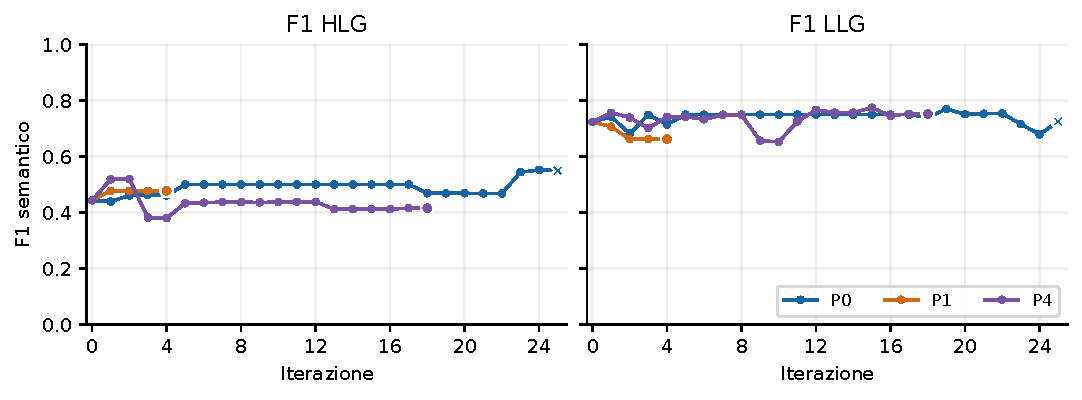
\includegraphics[width=\textwidth]{output/evaluation/thesis_completed_v103_20261025/iteration_trends/trend_auu.pdf}
\caption{Traiettorie F1 per AUU. L'iterazione 0 e la baseline; una croce indica arresto senza convergenza.}
\label{fig:iteration-trend-auu}
\end{figure}
\begin{table}[htbp]
\centering
\small
\caption{F1 dopo ogni iterazione per AUU. H: HLG; L: LLG.}
\label{tab:iteration-trend-auu}
\begin{tabular}{rrrrrrr}
\toprule
\textbf{Iter.} & \textbf{P0 H} & \textbf{P0 L} & \textbf{P1 H} & \textbf{P1 L} & \textbf{P4 H} & \textbf{P4 L} \\
\midrule
0 & 0,4435 & 0,7235 & 0,4435 & 0,7235 & 0,4435 & 0,7235 \\
1 & 0,4394 & 0,7424 & 0,4776 & 0,7072 & 0,5188 & 0,7565 \\
2 & 0,4612 & 0,6824 & 0,4776 & 0,6621 & 0,5197 & 0,7395 \\
3 & 0,4632 & 0,7494 & 0,4776 & 0,6621 & 0,3822 & 0,7015 \\
4 & 0,4611 & 0,7142 & 0,4776 & 0,6621 & 0,3801 & 0,7417 \\
5 & 0,5004 & 0,7497 & -- & -- & 0,4332 & 0,7423 \\
6 & 0,5004 & 0,7497 & -- & -- & 0,4355 & 0,7333 \\
7 & 0,5004 & 0,7497 & -- & -- & 0,4375 & 0,7487 \\
8 & 0,5004 & 0,7497 & -- & -- & 0,4375 & 0,7487 \\
9 & 0,5004 & 0,7497 & -- & -- & 0,4362 & 0,6566 \\
10 & 0,5004 & 0,7497 & -- & -- & 0,4374 & 0,6527 \\
11 & 0,5004 & 0,7497 & -- & -- & 0,4386 & 0,7253 \\
12 & 0,5004 & 0,7497 & -- & -- & 0,4386 & 0,7670 \\
13 & 0,5004 & 0,7497 & -- & -- & 0,4125 & 0,7572 \\
14 & 0,5004 & 0,7497 & -- & -- & 0,4125 & 0,7572 \\
15 & 0,5004 & 0,7497 & -- & -- & 0,4125 & 0,7745 \\
16 & 0,5004 & 0,7497 & -- & -- & 0,4125 & 0,7462 \\
17 & 0,5004 & 0,7497 & -- & -- & 0,4157 & 0,7526 \\
18 & 0,4690 & 0,7406 & -- & -- & 0,4157 & 0,7526 \\
19 & 0,4690 & 0,7696 & -- & -- & -- & -- \\
20 & 0,4690 & 0,7515 & -- & -- & -- & -- \\
21 & 0,4683 & 0,7532 & -- & -- & -- & -- \\
22 & 0,4683 & 0,7544 & -- & -- & -- & -- \\
23 & 0,5441 & 0,7158 & -- & -- & -- & -- \\
24 & 0,5523 & 0,6792 & -- & -- & -- & -- \\
25 & 0,5502 & 0,7255 & -- & -- & -- & -- \\
\bottomrule
\end{tabular}
\end{table}

\clearpage
\subsection{Fitness Tracker}
P0: 10 iterazioni, convergenza; P1: 3 iterazioni, convergenza; P4: 25 iterazioni, limite raggiunto.
\begin{figure}[htbp]
\centering
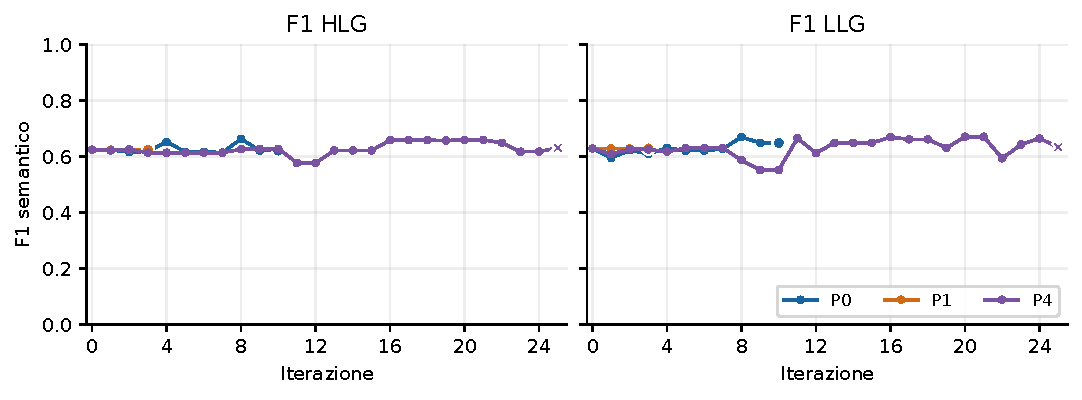
\includegraphics[width=\textwidth]{output/evaluation/thesis_completed_v103_20261025/iteration_trends/trend_fitness.pdf}
\caption{Traiettorie F1 per Fitness Tracker. L'iterazione 0 e la baseline; una croce indica arresto senza convergenza.}
\label{fig:iteration-trend-fitness}
\end{figure}
\begin{table}[htbp]
\centering
\small
\caption{F1 dopo ogni iterazione per Fitness Tracker. H: HLG; L: LLG.}
\label{tab:iteration-trend-fitness}
\begin{tabular}{rrrrrrr}
\toprule
\textbf{Iter.} & \textbf{P0 H} & \textbf{P0 L} & \textbf{P1 H} & \textbf{P1 L} & \textbf{P4 H} & \textbf{P4 L} \\
\midrule
0 & 0,6244 & 0,6288 & 0,6244 & 0,6288 & 0,6244 & 0,6288 \\
1 & 0,6244 & 0,5952 & 0,6244 & 0,6288 & 0,6221 & 0,6085 \\
2 & 0,6156 & 0,6227 & 0,6244 & 0,6288 & 0,6254 & 0,6265 \\
3 & 0,6178 & 0,6098 & 0,6244 & 0,6288 & 0,6138 & 0,6259 \\
4 & 0,6525 & 0,6308 & -- & -- & 0,6138 & 0,6174 \\
5 & 0,6173 & 0,6212 & -- & -- & 0,6138 & 0,6302 \\
6 & 0,6173 & 0,6212 & -- & -- & 0,6138 & 0,6302 \\
7 & 0,6140 & 0,6277 & -- & -- & 0,6138 & 0,6302 \\
8 & 0,6634 & 0,6699 & -- & -- & 0,6265 & 0,5873 \\
9 & 0,6215 & 0,6488 & -- & -- & 0,6278 & 0,5520 \\
10 & 0,6215 & 0,6488 & -- & -- & 0,6278 & 0,5520 \\
11 & -- & -- & -- & -- & 0,5775 & 0,6653 \\
12 & -- & -- & -- & -- & 0,5775 & 0,6126 \\
13 & -- & -- & -- & -- & 0,6219 & 0,6493 \\
14 & -- & -- & -- & -- & 0,6219 & 0,6493 \\
15 & -- & -- & -- & -- & 0,6219 & 0,6493 \\
16 & -- & -- & -- & -- & 0,6586 & 0,6691 \\
17 & -- & -- & -- & -- & 0,6586 & 0,6617 \\
18 & -- & -- & -- & -- & 0,6586 & 0,6617 \\
19 & -- & -- & -- & -- & 0,6576 & 0,6311 \\
20 & -- & -- & -- & -- & 0,6594 & 0,6709 \\
21 & -- & -- & -- & -- & 0,6594 & 0,6709 \\
22 & -- & -- & -- & -- & 0,6493 & 0,5938 \\
23 & -- & -- & -- & -- & 0,6174 & 0,6431 \\
24 & -- & -- & -- & -- & 0,6179 & 0,6645 \\
25 & -- & -- & -- & -- & 0,6313 & 0,6338 \\
\bottomrule
\end{tabular}
\end{table}

\clearpage
\subsection{La Reine Marlene}
P0: 13 iterazioni, convergenza; P1: 1 iterazioni, convergenza; P4: 3 iterazioni, convergenza.
\begin{figure}[htbp]
\centering
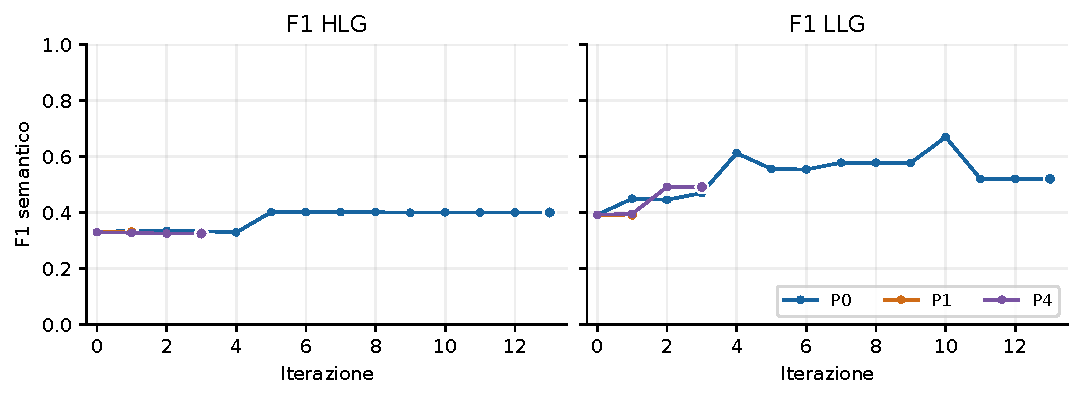
\includegraphics[width=\textwidth]{output/evaluation/thesis_completed_v103_20261025/iteration_trends/trend_marlene.pdf}
\caption{Traiettorie F1 per La Reine Marlene. L'iterazione 0 e la baseline; una croce indica arresto senza convergenza.}
\label{fig:iteration-trend-marlene}
\end{figure}
\begin{table}[htbp]
\centering
\small
\caption{F1 dopo ogni iterazione per La Reine Marlene. H: HLG; L: LLG.}
\label{tab:iteration-trend-marlene}
\begin{tabular}{rrrrrrr}
\toprule
\textbf{Iter.} & \textbf{P0 H} & \textbf{P0 L} & \textbf{P1 H} & \textbf{P1 L} & \textbf{P4 H} & \textbf{P4 L} \\
\midrule
0 & 0,3299 & 0,3923 & 0,3299 & 0,3923 & 0,3299 & 0,3923 \\
1 & 0,3355 & 0,4494 & 0,3299 & 0,3923 & 0,3279 & 0,3955 \\
2 & 0,3349 & 0,4455 & -- & -- & 0,3249 & 0,4913 \\
3 & 0,3335 & 0,4699 & -- & -- & 0,3249 & 0,4913 \\
4 & 0,3290 & 0,6122 & -- & -- & -- & -- \\
5 & 0,4015 & 0,5560 & -- & -- & -- & -- \\
6 & 0,4015 & 0,5540 & -- & -- & -- & -- \\
7 & 0,4015 & 0,5781 & -- & -- & -- & -- \\
8 & 0,4015 & 0,5781 & -- & -- & -- & -- \\
9 & 0,3996 & 0,5773 & -- & -- & -- & -- \\
10 & 0,4008 & 0,6697 & -- & -- & -- & -- \\
11 & 0,4003 & 0,5208 & -- & -- & -- & -- \\
12 & 0,4003 & 0,5208 & -- & -- & -- & -- \\
13 & 0,4003 & 0,5208 & -- & -- & -- & -- \\
\bottomrule
\end{tabular}
\end{table}

\clearpage
\subsection{London Ambulance Service}
P0: 6 iterazioni, convergenza; P1: 4 iterazioni, convergenza; P4: 13 iterazioni, convergenza.
\begin{figure}[htbp]
\centering
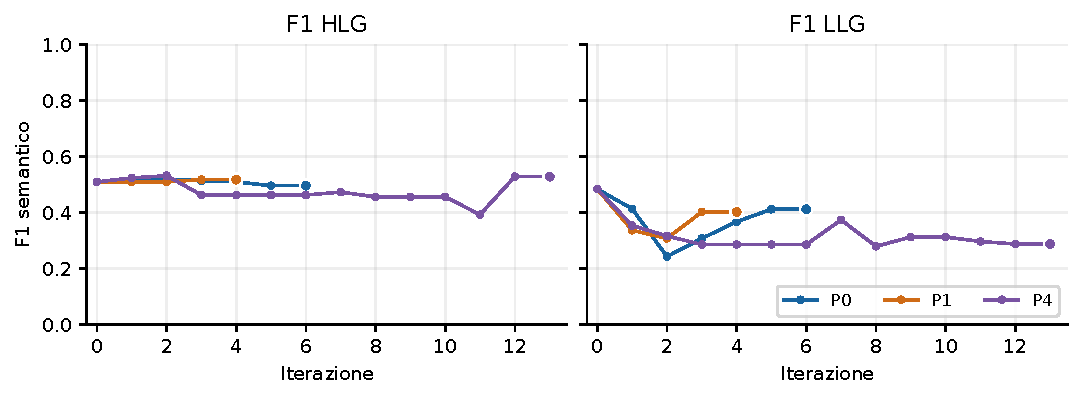
\includegraphics[width=\textwidth]{output/evaluation/thesis_completed_v103_20261025/iteration_trends/trend_london.pdf}
\caption{Traiettorie F1 per London Ambulance Service. L'iterazione 0 e la baseline; una croce indica arresto senza convergenza.}
\label{fig:iteration-trend-london}
\end{figure}
\begin{table}[htbp]
\centering
\small
\caption{F1 dopo ogni iterazione per London Ambulance Service. H: HLG; L: LLG.}
\label{tab:iteration-trend-london}
\begin{tabular}{rrrrrrr}
\toprule
\textbf{Iter.} & \textbf{P0 H} & \textbf{P0 L} & \textbf{P1 H} & \textbf{P1 L} & \textbf{P4 H} & \textbf{P4 L} \\
\midrule
0 & 0,5095 & 0,4841 & 0,5095 & 0,4841 & 0,5095 & 0,4841 \\
1 & 0,5169 & 0,4134 & 0,5095 & 0,3368 & 0,5239 & 0,3536 \\
2 & 0,5201 & 0,2429 & 0,5095 & 0,3077 & 0,5317 & 0,3164 \\
3 & 0,5134 & 0,3077 & 0,5176 & 0,4023 & 0,4628 & 0,2859 \\
4 & 0,5098 & 0,3675 & 0,5176 & 0,4023 & 0,4628 & 0,2859 \\
5 & 0,4960 & 0,4118 & -- & -- & 0,4628 & 0,2859 \\
6 & 0,4960 & 0,4118 & -- & -- & 0,4628 & 0,2859 \\
7 & -- & -- & -- & -- & 0,4732 & 0,3739 \\
8 & -- & -- & -- & -- & 0,4560 & 0,2793 \\
9 & -- & -- & -- & -- & 0,4560 & 0,3127 \\
10 & -- & -- & -- & -- & 0,4560 & 0,3127 \\
11 & -- & -- & -- & -- & 0,3927 & 0,2968 \\
12 & -- & -- & -- & -- & 0,5284 & 0,2877 \\
13 & -- & -- & -- & -- & 0,5284 & 0,2877 \\
\bottomrule
\end{tabular}
\end{table}

\clearpage
\subsection{Planning Poker}
P0: 11 iterazioni, convergenza; P1: 12 iterazioni, convergenza; P4: 9 iterazioni, convergenza.
\begin{figure}[htbp]
\centering
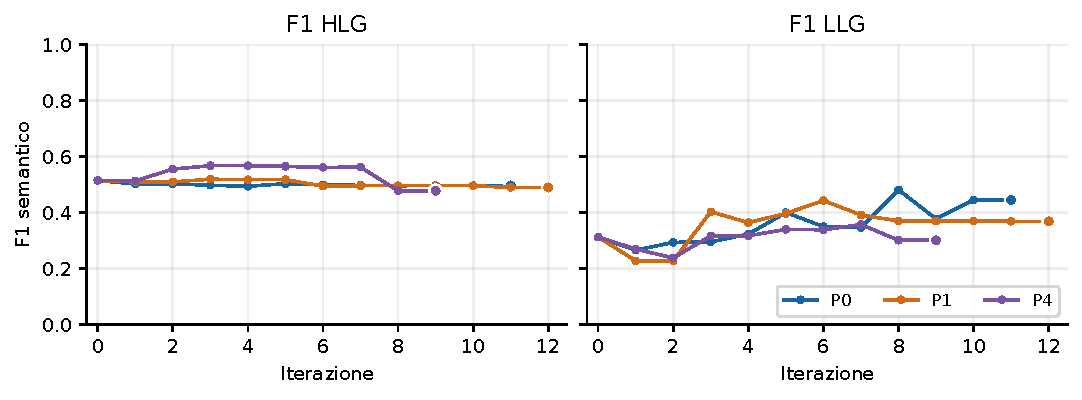
\includegraphics[width=\textwidth]{output/evaluation/thesis_completed_v103_20261025/iteration_trends/trend_poker.pdf}
\caption{Traiettorie F1 per Planning Poker. L'iterazione 0 e la baseline; una croce indica arresto senza convergenza.}
\label{fig:iteration-trend-poker}
\end{figure}
\begin{table}[htbp]
\centering
\small
\caption{F1 dopo ogni iterazione per Planning Poker. H: HLG; L: LLG.}
\label{tab:iteration-trend-poker}
\begin{tabular}{rrrrrrr}
\toprule
\textbf{Iter.} & \textbf{P0 H} & \textbf{P0 L} & \textbf{P1 H} & \textbf{P1 L} & \textbf{P4 H} & \textbf{P4 L} \\
\midrule
0 & 0,5147 & 0,3126 & 0,5147 & 0,3126 & 0,5147 & 0,3126 \\
1 & 0,5019 & 0,2658 & 0,5095 & 0,2276 & 0,5133 & 0,2695 \\
2 & 0,5026 & 0,2935 & 0,5095 & 0,2276 & 0,5553 & 0,2381 \\
3 & 0,4976 & 0,2952 & 0,5192 & 0,4027 & 0,5676 & 0,3171 \\
4 & 0,4940 & 0,3231 & 0,5175 & 0,3642 & 0,5676 & 0,3171 \\
5 & 0,5033 & 0,4001 & 0,5175 & 0,3967 & 0,5650 & 0,3400 \\
6 & 0,4988 & 0,3498 & 0,4946 & 0,4430 & 0,5614 & 0,3385 \\
7 & 0,4972 & 0,3468 & 0,4961 & 0,3914 & 0,5621 & 0,3574 \\
8 & 0,4959 & 0,4814 & 0,4961 & 0,3700 & 0,4781 & 0,3011 \\
9 & 0,4965 & 0,3774 & 0,4961 & 0,3700 & 0,4781 & 0,3011 \\
10 & 0,4965 & 0,4449 & 0,4961 & 0,3700 & -- & -- \\
11 & 0,4965 & 0,4449 & 0,4897 & 0,3687 & -- & -- \\
12 & -- & -- & 0,4897 & 0,3687 & -- & -- \\
\bottomrule
\end{tabular}
\end{table}

\clearpage
\subsection{SIA Project 25 26}
P0: 25 iterazioni, convergenza; P1: 4 iterazioni, convergenza; P4: 25 iterazioni, limite raggiunto.
\begin{figure}[htbp]
\centering
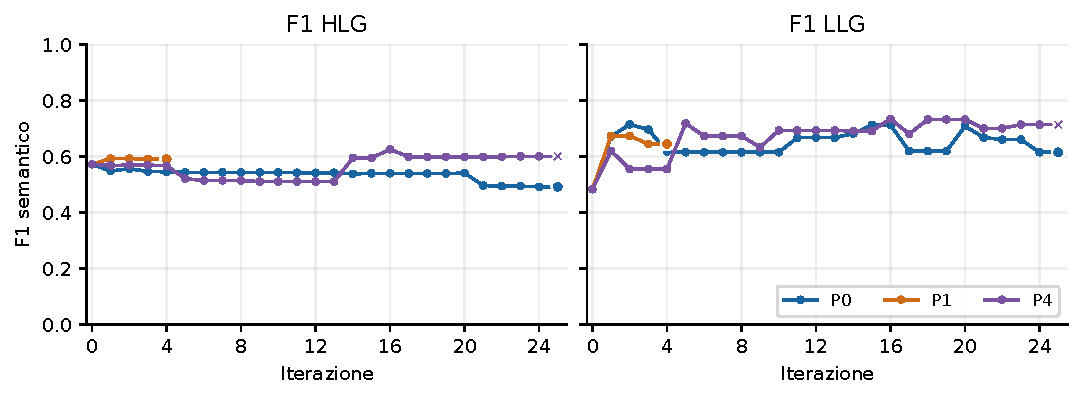
\includegraphics[width=\textwidth]{output/evaluation/thesis_completed_v103_20261025/iteration_trends/trend_sia.pdf}
\caption{Traiettorie F1 per SIA Project 25 26. L'iterazione 0 e la baseline; una croce indica arresto senza convergenza.}
\label{fig:iteration-trend-sia}
\end{figure}
\begin{table}[htbp]
\centering
\small
\caption{F1 dopo ogni iterazione per SIA Project 25 26. H: HLG; L: LLG.}
\label{tab:iteration-trend-sia}
\begin{tabular}{rrrrrrr}
\toprule
\textbf{Iter.} & \textbf{P0 H} & \textbf{P0 L} & \textbf{P1 H} & \textbf{P1 L} & \textbf{P4 H} & \textbf{P4 L} \\
\midrule
0 & 0,5725 & 0,4833 & 0,5725 & 0,4833 & 0,5725 & 0,4833 \\
1 & 0,5484 & 0,6718 & 0,5930 & 0,6739 & 0,5680 & 0,6196 \\
2 & 0,5567 & 0,7150 & 0,5930 & 0,6739 & 0,5695 & 0,5555 \\
3 & 0,5469 & 0,6968 & 0,5911 & 0,6450 & 0,5695 & 0,5555 \\
4 & 0,5456 & 0,6181 & 0,5911 & 0,6450 & 0,5671 & 0,5552 \\
5 & 0,5435 & 0,6154 & -- & -- & 0,5212 & 0,7184 \\
6 & 0,5435 & 0,6154 & -- & -- & 0,5145 & 0,6733 \\
7 & 0,5435 & 0,6154 & -- & -- & 0,5145 & 0,6733 \\
8 & 0,5435 & 0,6154 & -- & -- & 0,5145 & 0,6733 \\
9 & 0,5435 & 0,6154 & -- & -- & 0,5108 & 0,6333 \\
10 & 0,5435 & 0,6154 & -- & -- & 0,5108 & 0,6935 \\
11 & 0,5423 & 0,6675 & -- & -- & 0,5108 & 0,6935 \\
12 & 0,5423 & 0,6675 & -- & -- & 0,5108 & 0,6935 \\
13 & 0,5423 & 0,6675 & -- & -- & 0,5108 & 0,6935 \\
14 & 0,5381 & 0,6821 & -- & -- & 0,5952 & 0,6913 \\
15 & 0,5401 & 0,7129 & -- & -- & 0,5952 & 0,6913 \\
16 & 0,5401 & 0,7129 & -- & -- & 0,6262 & 0,7345 \\
17 & 0,5396 & 0,6194 & -- & -- & 0,5993 & 0,6809 \\
18 & 0,5396 & 0,6194 & -- & -- & 0,5993 & 0,7325 \\
19 & 0,5396 & 0,6194 & -- & -- & 0,5993 & 0,7325 \\
20 & 0,5408 & 0,7088 & -- & -- & 0,5993 & 0,7325 \\
21 & 0,4966 & 0,6681 & -- & -- & 0,5993 & 0,7007 \\
22 & 0,4943 & 0,6609 & -- & -- & 0,5993 & 0,7007 \\
23 & 0,4943 & 0,6609 & -- & -- & 0,6010 & 0,7142 \\
24 & 0,4920 & 0,6153 & -- & -- & 0,6010 & 0,7142 \\
25 & 0,4920 & 0,6153 & -- & -- & 0,6010 & 0,7142 \\
\bottomrule
\end{tabular}
\end{table}

\clearpage
